%Vision is one of the most important senses for animals; humans use it extensively for all kinds of tasks. Hunting, assessing danger, reading, driving, drawing, predicting rain from grey clouds, etc., these are all tasks that involve \emph{seeing}. There is a vast collection of knowledge about the components of vision (primates in particular), though a unification (or the answer to \emph{How do we see?}) has not yet been achieved.

Artificial neural networks have already been used to emulate some functions of the human visual system. One of the most successful is image recognition, in particular using deep networks~\cite{deep-nets-hinton2006fast,krizhevsky2012imagenet}. Seminal computer vision research has also been based on the functional characteristics of biological vision, for example  \citeauthor{lowe1999object} devised an algorithm to obtain invariant features in images inspired by the retina~\cite{lowe1999object,lowe2004distinctive,alahi2012freak}. The success of bio-inspired research in computer vision is our inspiration for studying the visual pathway in animals (primates in particular) and to create a system that would solve the SLAM problem. In this chapter we shall review the visual pathway and artificial neural networks that have attempted to model it. 

\section{The eye and the retina}
\label{sec:vision:eye}
Our everyday experience might lead us to believe that the eyes are sensory organs developed completely separate from the brain but, in fact, the retina is an extension of the brain that performs spatio-temporal compression of a continuous flow of ``images'' of the world.

The eye is composed of many parts that resemble a camera (LENS, CAMERA OSCURA, FILM)

After light has been transformed into an electrical representation, the retina takes over and computes a representation of it.

Photoreceptors have the task of transforming light into an electrical signal. Colour is perceived by special type of receptors \emph{cones}. For low-light conditions and higher contrast sensitivity, we use \emph{rods}. Vertebrates have both rods and cones. Evolutionary adaptation has made eyes in different animals have special ratios of cones and rods. Reptiles and fish have more cones, most likely because they ``live'' on daytime for a lack of worm blood.

Many mammals have retinas with more rods than cones. For primates the retina has has two almost dual sensor zones. Most of the photosensitive area has more rods than cones; a tiny region called the \emph{foveal pit} has almost no rods, is densely packed with cones for high-resolution vision and is virtually blind when there is not enough light.

Horizontal cells average spatially (surround), input from photoreceptors; output to bipolar and to photoreceptors (adapt to different light conditions)

Bipolar cells, centre behaviour, input from horizontal and photoreceptors

IMAGE OF CENTRE SURROUND!!!!

First layers (photoreceptors, bipolar, horizontal cells) use analog signals, ganglion cells use spike trains.

Most authors agree that ganglion cells can be modelled by a \emph{Difference of Gaussians} due to its centre-surround behaviour.

Ganglion cells extend to the Lateral Geniculate Nucleus, where information is relayed and organized so that the cortex can interpret it. 

Organization makes left visual field sent to right hemisphere, right field to left hemisphere.



\section{The visual cortex}
\label{sec:vision:cortex}
The portion of the cortex that is involved with visual processing has been estimated to about 30\%.

It has been studied and areas have been labelled due to their function.

V1, V2, V...



\section{Artificial neural networks}
Artificial neural networks (ANN) first appeared as a novel way of solving problems that was inspired by the way the brain computes~\cite{mcculloch1943logical}. ANNs are graph models where nodes are model neurons and edges are weighed connections. In general, they learn statistics about their inputs through a learning algorithm that adjusts the weights of the edges, akin to synaptic plasticity. They have been widely used to solve problems such as classification, pattern recognition, function approximation, to name a few.

Generations of neural networks can be classified by their basic compute unit, the neuron model. Under this scheme, the \textbf{first generation} used \textsc{on-off} threshold gates, also known as perceptrons~\cite{minsky1987perceptrons}. The basic functionality is that if the input value is above a certain threshold, the neuron will output a 1, otherwise a 0. First generation ANN are able to compute every boolean function using a single hidden layer~\cite{third-gen-nn-Maass1997}.

The \textbf{second generation} of neural models make use of an activation function which enables the output of analog values. The typical activation function is a sigmoid (eq. \ref{eq:neuro:sigmoid}). Whenever the activation function reaches a certain threshold, the neuron will be ``fire''.

\begin{equation}
  \sigma(x) = \frac{1}{1 + e^{-x}}
  \label{eq:neuro:sigmoid}
\end{equation}
\vspace*{0.1cm}

A notable addition is that multi-layered network of the second generation are able to be trained using gradient descent-based algorithms~\cite{hecht1989-backprop-theory}. They can be interpreted as neurons using rate coding which is an unlikely candidate for fast computations in the brain~\cite{third-gen-nn-Maass1997}.

\emph{Spiking neural networks} are considered the \textbf{third generation} of ANN, the main difference is that their activation function is closer to the one observed in biological neurons. Some neuron models used were described in Section~\ref{sec:brain:neurons}. Third generation ANN are able to approximate any analog continuous function~\cite{third-gen-nn-Maass1997}. 
%\begin{figure}
%  \begin{center}
%    \begin{subfigure}{0.25\textwidth}
%      %    \vspace*{0.8em}
%      \centering
%      \captionsetup{justification=centering}
%      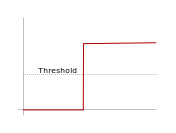
\includegraphics[width=\textwidth]{perceptron}
%      \caption{Perceptron}
%      \label{fig:neuro:perceptron}
%    \end{subfigure}
%    \begin{subfigure}{0.25\textwidth}
%      %    \vspace*{0.8em}
%      \centering
%      \captionsetup{justification=centering}
%      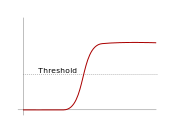
\includegraphics[width=\textwidth]{sigmoid}
%      \caption{Sigmoid}
%      \label{fig:neuro:sigmoid}
%    \end{subfigure}
%    \begin{subfigure}{0.265\textwidth}
%      \centering
%      \captionsetup{justification=centering}
%      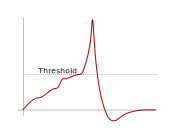
\includegraphics[width=\textwidth]{spike}
%      \caption{Spike}
%      \label{fig:neuro:spike-func}
%    \end{subfigure}
%  \end{center}
%\end{figure}
There are some synaptic learning rules for spiking neural networks, the most studied one being Spike-Timing-Dependant Plasticity (STDP)~\cite{STDP-Song2000}. 
It follows a Hebbian philosophy, \emph{neurons that fire together, wire together}~\cite{hebb2005organization}. The basic idea is that when a post-synaptic spike is generated nearly after a pre-synaptic one, the connection is between this pre and post neurons is strengthened.\\

If network topology is also taken into the classification basis, a new generation can be added. \emph{Deep networks} are thought to be the \textbf{fourth generation} of neural networks. Previously, researchers had tried to train deep networks but found that it was a difficult task to achieve for more than one-hidden-layered networks and it actually decreased the performance of the network~\cite{learning-deep-Bengio2009}. In 2006, \citeauthor{hinton2006fast} reported an algorithm to train deep architectures without supervision, one layer at a time; the authors named their network a \emph{Deep Belief Network} (DBN)~\cite{hinton2006fast}. After this seminal work, other researchers used the same one layer at a time  approach but with different learning algorithms. While \citeauthor{hinton2006fast} used restricted Boltman machines (RBM), \citeauthor{autoencoders-lecun2007} used auto-encoders~\cite{autoencoders-lecun2007}. Since these learning techniques are being used with non-spiking neural networks, the use of deep architectures in SNN has been limited. The usual path is to train a network off-line, transfer the weights to an equivalent SNN and use that as the energy-efficient on-line application~\cite{evangelos-deep-belief,diehlfast-deep-net}.

\section{Visual cortex models}
Classical computer vision has limitations and is not near the performance of the human visual system. The use of ANN for image recognition has recently shown successful results~\cite{krizhevsky2012imagenet}. Unfortunately this is just one of the many functions of the visual system, to the best of our knowledge, most models of visual functions are based in a few parts of the visual cortex. For some tasks (e.g. image recognition), most models are using a feed-forward approach but that doesn't account for any of the back projections observed in the brain.

An observed characteristic in the visual system is the use of simple and complex cells, which are present in different layers along the visual cortex~\cite{hubel1962receptive,thompson2000brain}. The presence of these cells could explain the preferred activation of some neurons to bars in a certain orientation. Simple cells receive information from one or more neurons coming the retina and the LGN. Complex cells' inputs come from one or more simple cells, allowing them to respond to a particular orientation in a region of the retina. Figure~\ref{fig:vision:simple-complex} shows an example of the connectivity of simple and complex cells.

\begin{figure}[h]
  \begin{center}
    \begin{subfigure}[t]{0.4\textwidth}
      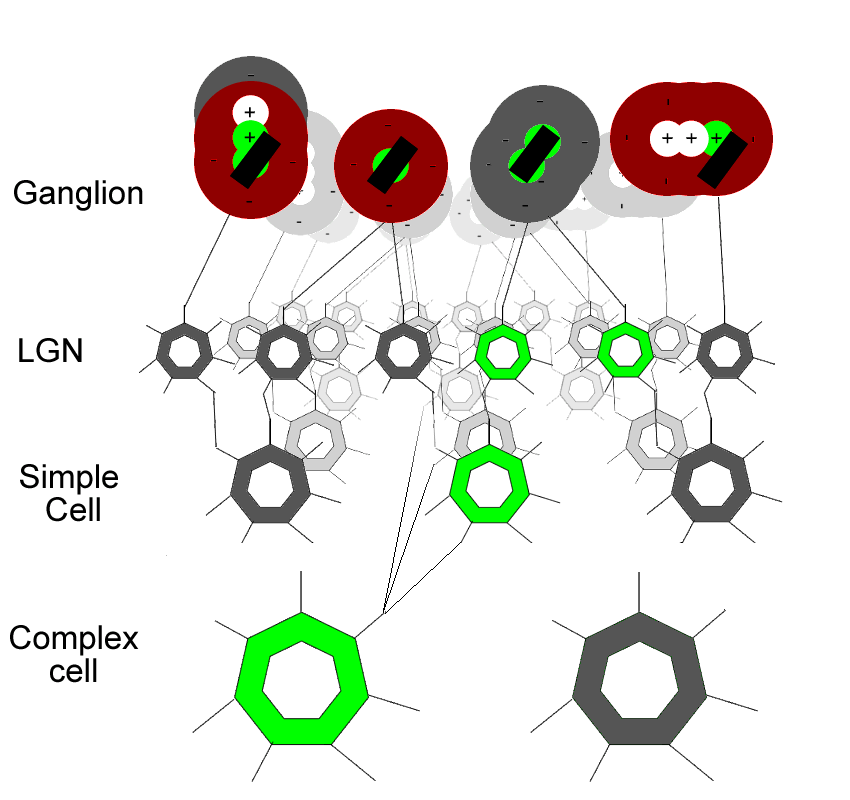
\includegraphics[width=\textwidth]{simple-complex-diag-bar}
      \caption{Response to a diagonal bar.}
    \end{subfigure}
    \begin{subfigure}[t]{0.4\textwidth}
      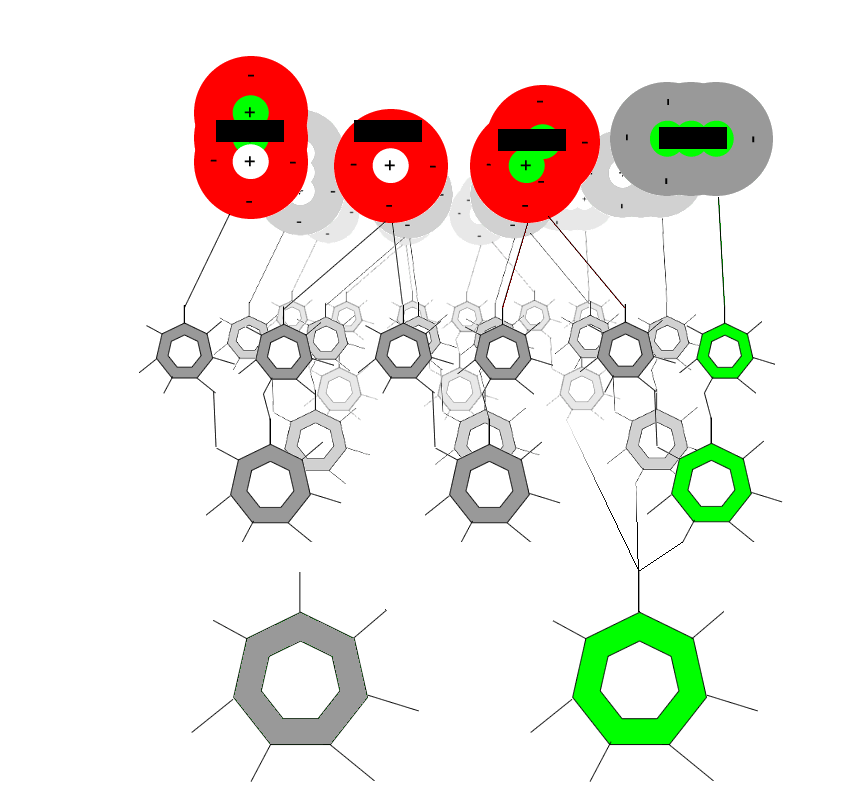
\includegraphics[width=\textwidth]{simple-complex-horiz-bar}
      \caption{Response to a horizontal bar.}
    \end{subfigure}
    \caption{Diagrams of the simple and complex cells (adapted from~\cite{wikipedia-images}). }
    \label{fig:vision:simple-complex}
  \end{center}
\end{figure}

Some models make use of hierarchical topologies that resemble the organization of the visual cortex. The main idea behind a hierarchy is that successive layers encode more complex patterns than the previous one. For example, Figure~\ref{fig:vision:hierarchical_encoding} shows a fictional network whose units in the first layer respond to oriented edges. The next layer has a preference for corners and, finally, the third layer responds better to shapes.

\begin{figure}[h]
  \begin{center}
    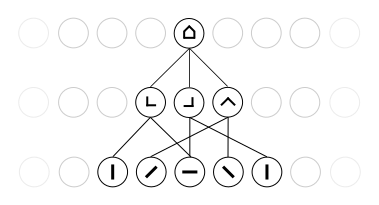
\includegraphics[width=0.5\textwidth]{hierarchical_encoding}
    \caption{Progressively more complex features in each successive layer.}
    \label{fig:vision:hierarchical_encoding}
  \end{center}
\end{figure}

The Neocognitron is an example of a hierarchical topology which uses the simple-complex cell concept~\cite{fukushima1988neocognitron}; simple cells from one layer sample from complex cells in the previous. The downside of this model is that it has been proven to be hard to train.

A variation of the simple-complex cell architecture is known as HMAX~\cite{riesenhuber1999hierarchical}. The simple cells perform template matching through a weighed sum of their input and the complex a softmax operation. The softmax operation selects the best candidate of the simple cells and transmits that to the next layer.

Yet another adaptation of the simple-complex architecture is used in Convolutional Networks~\cite{lecun-1990handwritten}. Here, complex cells perform a convolution of their inputs and simple cells sub-sample the output of complex cells.

Hierarchical networks have been shown to provide geometric transformation invariance, though most examples only model feed-forward connectivity. Recurrent networks are among the few that use feed-back in their design. Though they might be difficult to use due to unwanted interactions between layers. They have been used successfully for spatio-temporal pattern and hand-written text recognition, and motor control. A model known as \emph{LAMINART} makes use of feedback connections, and it's based the laminar circuits of the cortex~\cite{raizada2003laminart}. The model is biologically plausible and has been adapted to simulate different perceptual effects. The \emph{Neural Abstraction Pyramid} architecture is another model that is bio-inspired and uses lateral and feedback connections~\cite{behnke2003hierarchical}. It's been used for various visual tasks such as image recognition and face localization.


\section{Conclusions}
\label{sec:vision:conclusions}
A complete model the visual cortex remains an open research question. Though many neural networks and computer vision models account for single visual functions, a unified solution has not been developed. Since environment reconstruction makes use of many of these functions, this research could lead to contributions to a general theory of vision. 

A hierarchical neural networks approach promises to have better results. The training of deep spiking neural networks is still in early stages of research, which brings another opportunity for contributions to neuroscience. Recurrent neural networks could provide the necessary framework to solve the training problem.
